\documentclass[14pt,fleqn]{extarticle}
\RequirePackage{prepwell}

\previewoff

\newcommand\expa{16- \left(x-4 \right)^2}
\newcommand\intga{\int_0^4 \sqrt{\expa}\cdot dx}
\newcommand\intgb{2\int_0^4 \sqrt{x}\cdot dx}


\begin{document} 

\begin{question}
	\statement 
    
     Using integration, find the area lying above the \xaxis and included between the circle $x^2 + y^2 = 8x$ and the parabola $y^2 = 4x$ 
     
     \begin{step}
  \begin{options} 
     \correct 
       
     The circle is centered at $C = \left(4,0 \right)$ and has radius $R = 4$ as shown below 

     \begin{center}
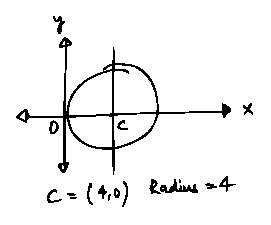
\includegraphics[scale=1.2]{1381-A.eps}
\end{center}
     \incorrect
     
          The circle is centered at $C = \left(0,0 \right)$ and has radius $R = \sqrt{8} = 2\sqrt{2}$ as shown below 
        
        \begin{center}
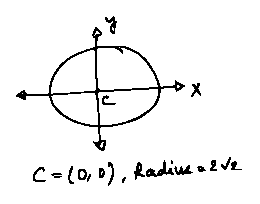
\includegraphics[scale=1.2]{1381-B.eps}
\end{center}
    \end{options} 
     \reason 
     
     The equation we have been given for the circle is \underline{not} in the 
     standard form. Hence, we must first make it so
     
     \begin{align}
x^2 + y^2 &= 8x \\
\left(x^2-8x \right)	 + y^2 &= 0 \\
\underbrace{\left(x^2-8x + 16 \right)}_{\text{Completing the squares}} &+ y^2 - 16 = 0 \\
\left(x-4 \right)^2 + y^2 &= 16 
\end{align}
       
       Now, it is in standard form. And we can see that the circle's center is at $C = \left(4,0 \right)$ and it's radius is $R = \sqrt{16} = 4$. Hence, the circle would look like this 
       
       \begin{center}
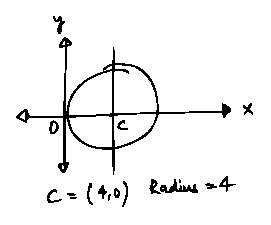
\includegraphics[scale=1.2]{1381-A.eps}
\end{center}
\end{step} 

\begin{step}
  \begin{options} 
     \correct 
       
       \begin{center}
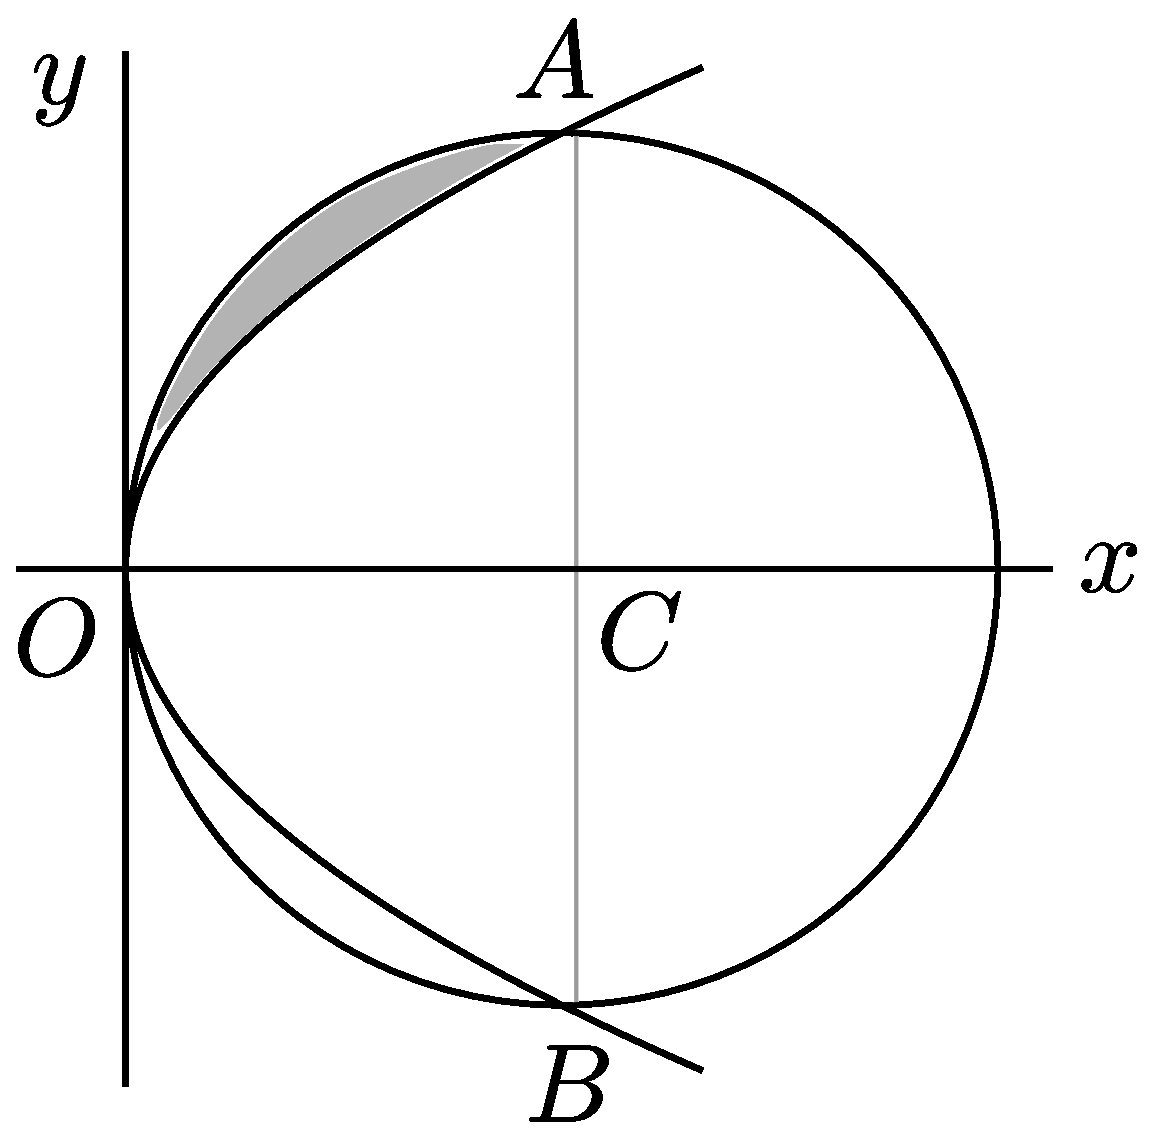
\includegraphics[scale=0.2]{1381-C.eps}
\end{center}

$A = \left(4,4 \right)$ and the shaded portion is the required area 
     \incorrect
        
        \begin{center}
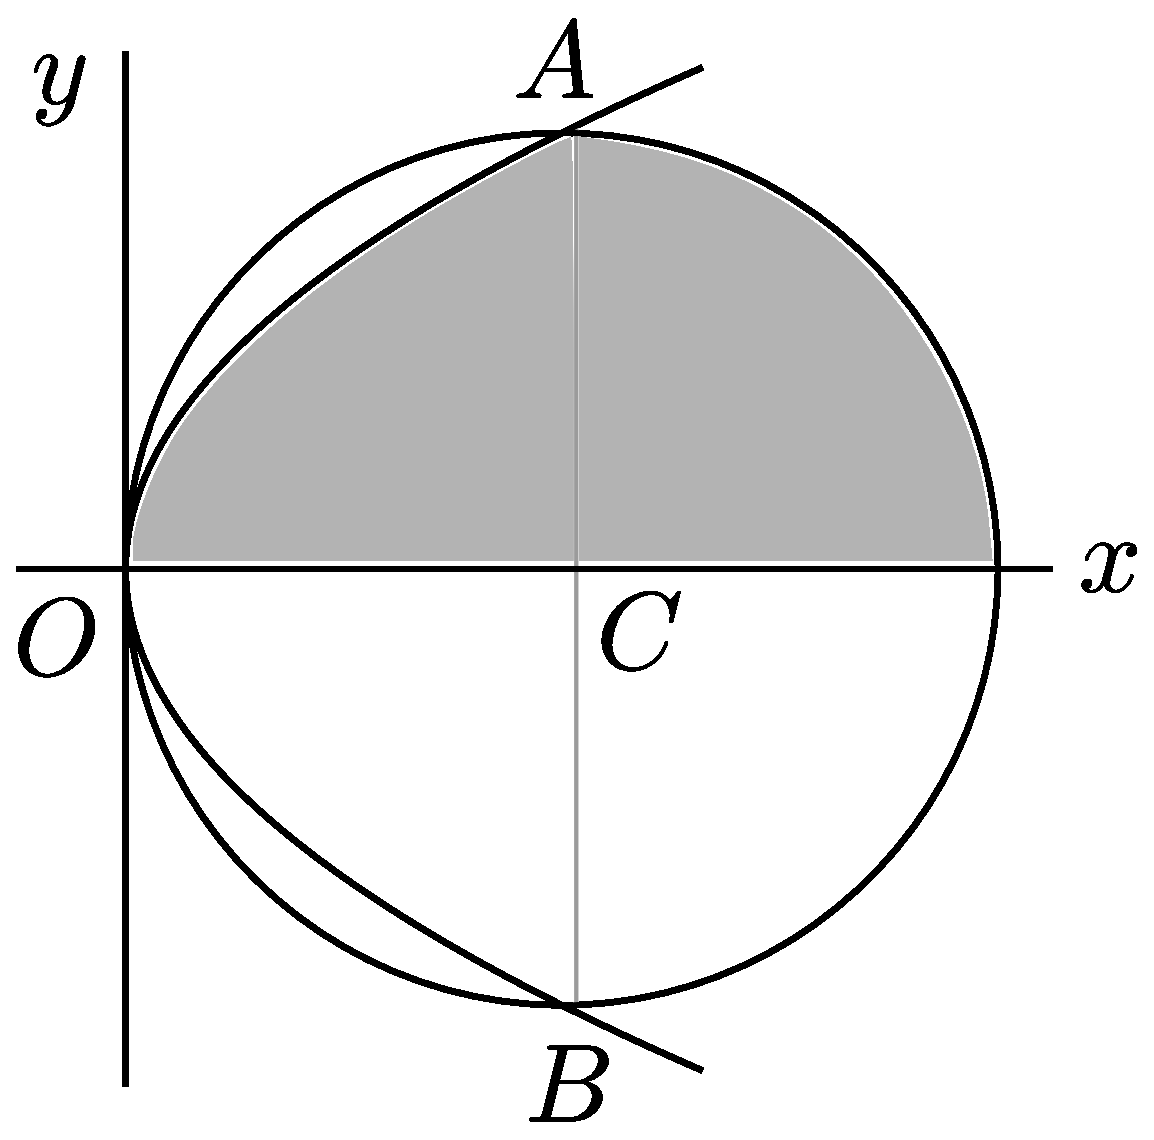
\includegraphics[scale=0.2]{1381-D.eps}
\end{center}

$A = \left(4,4 \right)$ and the shaded portion is the required area 
    \end{options} 
     \reason 
     
     The parabola is \underline{initially inside the circle}. How do we know 
     that? Well, just find the $y$ for both the circle and the parabola 
     when $x=1$. The curve for which $y$ is \underline{higher} is outside\newline 
     
     Now, the two curves will intersect when 
     
     \begin{align}
     y^2 = 4x = \underbrace{8x-x^2}_{\text{Circle}}&\text{ or } x^2 - 4x = 0  \\
     \implies x\cdot \left(x-4 \right) &= 0\text{ or } x = 0,4 
\end{align}

Which gives us \underline{three} points of intersection -- $O = (0,0), A = (4,4)$ and $B=(4,-4)$ \newline 

But the required area must be \underline{above} the \xaxis and \underline{between} the two curves. Hence, it would be as shown 

\begin{center}
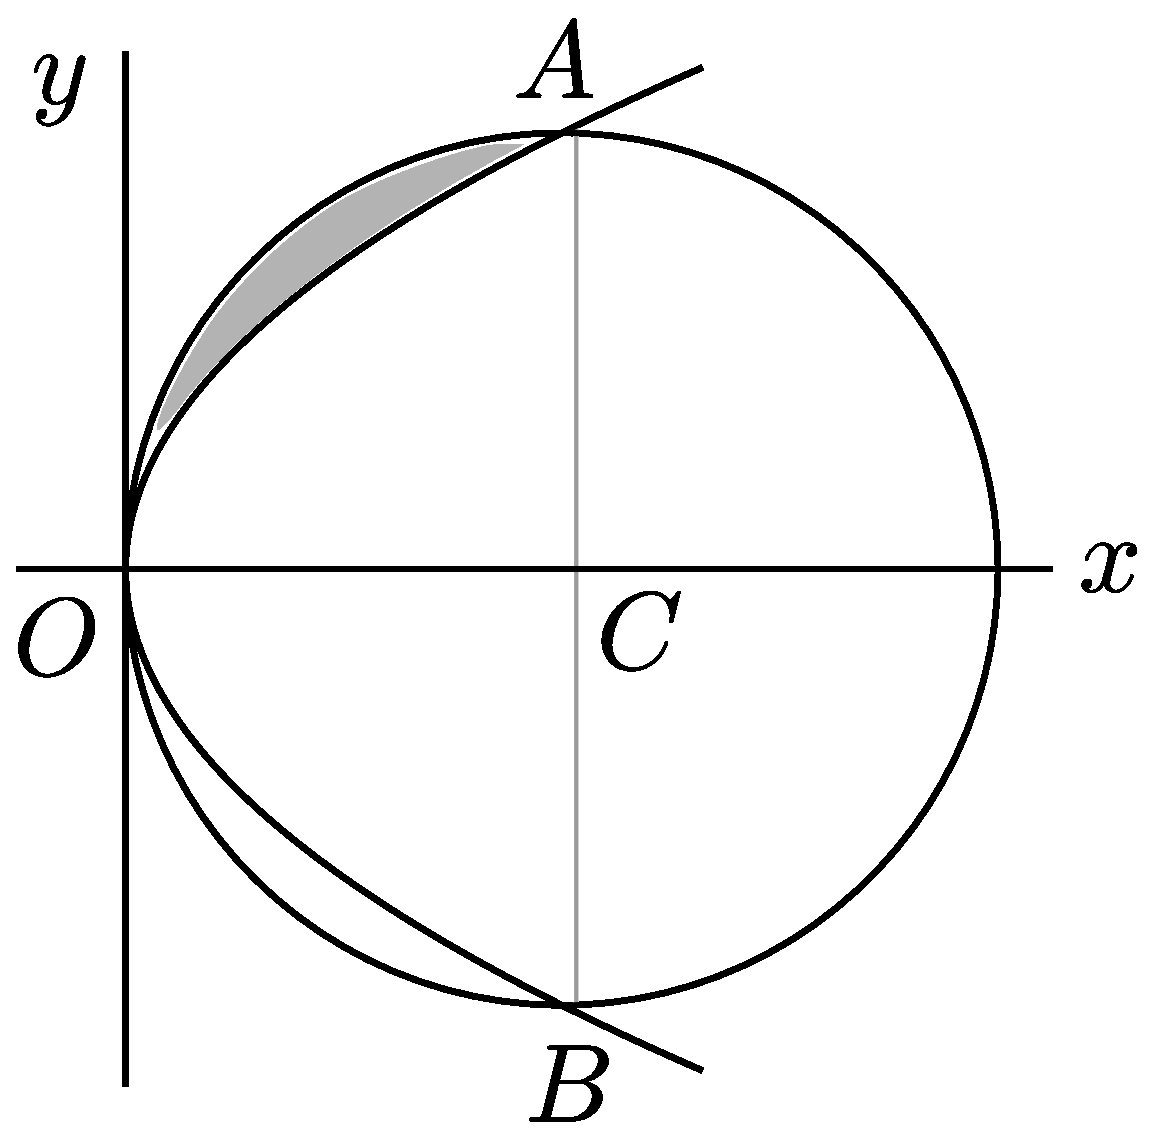
\includegraphics[scale=0.2]{1381-C.eps}
\end{center}
       
\end{step}

\begin{step}
  \begin{options} 
     \correct 
       
     The required area $R$ will be 
     \smallmath
     \begin{align}
	R &= \intga - \intgb \\
	&= \left[\frac{x-4}{2}\sqrt{\expa} + 8\sin^{-1}\frac{x-4}{4} - \frac{4}{3}x^{\frac{3}{2}}\right]_0^4 \\
	&= 4\pi - \frac{32}{3}
\end{align}

  
    \end{options} 
     \reason 
     
     From the figure we can see that 
     \smallmath\begin{align}
     R &= \underbrace{\intga}_{\text{Under the circle}} - \underbrace{\int_0^4 \sqrt{4x}\cdot dx}_{\text{Under the parabola}} \\
     &= \underbrace{\intga}_M - \underbrace{\intgb}_N
\end{align}

Now, in $M$ if $z = x-4$, then $dz = dx$
\smallmath\begin{align}
\text{So, } &\int \sqrt{\expa}\cdot dx = \int\sqrt{4^2-z^2}\cdot dz \\[-30pt]
&= \underbrace{\left[\frac{z}{2}\sqrt{16-z^2} + \frac{16}{2}\sin^{-1} \left(\frac{z}{4} \right) \right] + C}_{\int \sqrt{a^2 - z^2}\cdot dx = ?} \\
&= \left[\frac{x-4}{2}\sqrt{\expa} + 8\sin^{-1} \left(\frac{x-4}{4} \right) \right] + C \\
\therefore M &= \left[\frac{x-4}{2}\sqrt{\expa} + 8\sin^{-1} \left(\frac{x-4}{4} \right) \right]_0^4 \\
&= \left[\left(0+0 \right) - \left\lbrace 0 + 8\sin^{-1} \left(\frac{0-4}{4} \right)\right\rbrace \right] \\
&= -8\sin^{-1} \left(-1\right) = -8\cdot -\frac{\pi}{2} = 4\pi \\
N &= 2\int_0^4\sqrt{x} = 2 \left[\frac{x^{\frac{3}{2}}}{\frac{3}{2}} \right]_0^4 = \frac{4}{3} \left[x^{\frac{3}{2}} \right]_0^4  \\
&= \frac{4}{3} \left[4^{\frac{3}{2}} - 0 \right] = \frac{4}{3}\cdot 8 = \frac{32}{3} \\
R &= M - N = 4\pi - \frac{32}{3} \\
&\approx 4\cdot \frac{22}{7} - \frac{32}{3} = \frac{40}{21} \text{ (approximately)}
\end{align}
       
\end{step}
\end{question} 
\end{document} 